\documentclass{my-cv}

\author{David Jos\'{e} da Rocha Marques}
\title{Curriculum Vitae}
\date{\today{}}

% Enable for xelatex
\usepackage{fontspec}
    \setmainfont{Arial}

\begin{document}
\pagenumbering{gobble}          % No page numbering
\topinfo{
  Recent graduate interested in \emph{Data Science}/\emph{IT}. Highly motivated, very quick learner and extremely self-taught. Always eager to learn and improve, both personally and professionally. 
}                        % Name and stuff

\vspace{4mm}



\begin{tabular}{l|l}
\begin{minipage}[t][][b]{.35\linewidth}
    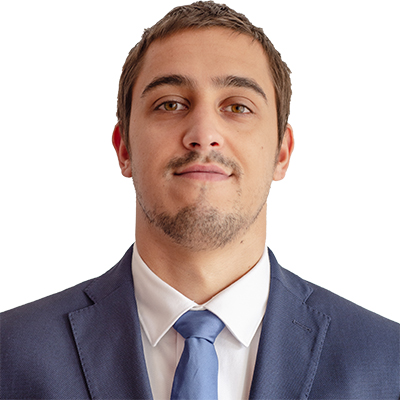
\includegraphics[width=\textwidth]{figures/david_2_linkdin.jpg} % Picture

    \vspace{2mm}

    \begin{skills}{Info}

    \nationality{Portuguese}

    \phone{+351 962 154 064}

    \email{davidmarques856@gmail.com}
    \vspace{3mm}
    \end{skills}
    % Here is the info

    \begin{skills}{Languages}

    \skillentry{Portuguese}{5}\\
    \skillentry{English}{5}\\
    \skillentry{German}{1}
    \end{skills}

    \begin{skills}{Programming}

    \skillentry{Python}{4}
    \skillentry{\LaTeX2}{4}
    \skillentry{Matlab}{3}
    \skillentry{\emph{SQL}}{2}
    \skillentry{Elisp}{2}
    \skillentry{Bash}{1}
    \skillentry{C}{1}
    \end{skills}



    \begin{skills}{Tools}
    \skillentry{Git}{3}
    \end{skills}

    \begin{skills}{Operative Systems}
    \skillentry{GNU/Linux}{4}\\
    \skillentry{Windows}{4}
    \end{skills}

    \begin{skills}{Commercial Software}
    \skillentry{Mcsft. Excel}{4}\\
    \skillentry{Mcsft. Word}{4}\\
    \skillentry{Mcsft. PwPt}{4}
    \end{skills}

    \begin{skills}{General Skills}
    \unratedskill{Team-work}\\
    \unratedskill{Communication}\\
    \end{skills}

    \begin{skills}{Hobbies}
    \unratedskill{Reading}\\
    \unratedskill{Traveling}\\
    \unratedskill{Programming}\\
    \end{skills}


\end{minipage}&
\begin{minipage}[t][][t]{.65\linewidth}

  % Education Bit
  \begin{cvpart}{Education}
    \experience{Mechanical Engineering Masters}{2011-2018}{Energy Department. \\ Instituto Superior T\'{e}cnico, Lisboa, Portugal. \\ Master's Grade Average: 15/20}
  \end{cvpart}

  \begin{cvpart}{Extracurricular Activities}
    \experience{JUNITEC}{2016-2017}{
      University's junior company. Member of the technical department, part of a team working directly in a project.}
    \devskills{Team-work, Communication, Event Organization }




    \experience{University Grant}{2017-2018}{
      Monitor of laboratory equipped with computers with technical software, used by students. Functions included guaranteeing good study conditions and proving support to other students regarding the usage of software related with programming, \emph{CAD}, and \emph{FEM}. \\
      Networking, account creation/administration, software and hardware maintenance of 60 divided in two rooms.}
    \devskills{Team-work, Communication, Management, Windows,\\ Networking}
  \end{cvpart}


  \begin{cvpart}{Notable Projects}
    \project{Master's Dissertation \hfill \normalfont{Grade: $18/20$}}{
      Intelligent thermal comfort controller capable of adapting to a office user's preference and autonomously managing the ventilation system.\\ Learning system based on Reinforcement Learning.}
    \devskills{Python, \emph{SQL}, Linux, Rasperry Pi, \LaTeX2, Git}

    \project{\emph{Techstorm} \hfill \normalfont{$2_{nd}$ Place}}{
      24 hours to develop an electronic product and present it in a 3 min pitch. The team was awarded the second place.
    }
    \devskills{Team-work, Communication, Python, Arduino}

    \project{Biogamming}{
      \emph{EMG} and arduino based product with the objective of controlling video games with muscle movement. 
    \devskills{Team-work, Communication, Python, Arduino}
    }

  \end{cvpart}

\end{minipage}
\end{tabular}
\end{document}

%%% Local Variables: 
%%% coding: utf-8
%%% mode: latex
%%% TeX-engine: xetex
%%% End: 

